%!TEX encoding = UTF-8 Unicode

\documentclass[aspectratio=1610, polish]{beamer}
\usetheme{Warsaw}

\usecolortheme{crane}

\usepackage[T1]{fontenc}
\usepackage{polski}
\usepackage{listingsutf8}
\usepackage{tikz}

\usepackage{fontspec}
\setmainfont{Carlito}
\usepackage{macros}
\usepackage{subcaption}

\lstset{
    language=Python,                % choose the language of the code
    basicstyle=\ttfamily,           % the fonts that are used for the code
    numbers=left,                   % where to put the line-numbers
    numberstyle=\footnotesize,      % the size of the fonts that are used for the line-numbers
    stepnumber=1,                   % the step between two line-numbers. If it's 1 each line will be
    numbersep=5pt,                  % how far the line-numbers are from the code
    showspaces=false,               % show spaces adding particular underscores
    showstringspaces=false,         % underline spaces within strings
    showtabs=false,                 % show tabs within strings adding particular underscores
    frame=single,                   % adds a frame around the code
    tabsize=4,                      % sets default tabsize to 2 spaces
    captionpos=b,                   % sets the caption-position to bottom
    breaklines=true,                % sets automatic line breaking
    breakatwhitespace=false,        % sets if automatic breaks should only happen at whitespace
    %postbreak=\mbox{\textcolor{red}{$\hookrightarrow$}\space},
    escapeinside={\%*}{*)},         % if you want to add a comment within your code
    % custom python colors
    commentstyle=\color{green},
    stringstyle=\color{purple},
    numberstyle=\footnotesize\color{gray},
    emph={main,process_raw_data,minmax_normalize,create_model_ssn,create_model_rsn,timeseries_dataset_from_array,gen_plot},
    emphstyle=\bfseries\color{orange},
    morekeywords={
        with
    },
    keywordstyle=\bfseries\color{violet},
    keywordstyle=[2]\bfseries\color{cyan},
    keywordstyle=[3]\bfseries\color{blue},
    morekeywords=[2]{
        json,csv,path,environ,pd,plt,ticker,MultipleLocator,Axes,LSTM,Dense,Adam,MeanSquaredError,
        Exception,datetime
    },
    deletekeywords = {def, global, not, or, True, False},
    morekeywords=[3]{
        def, global, not, or, True, False
    }
}

\title{Efektywność SMT solverów dla klasycznych problemów NP-trudnych}
\subtitle{Effectiveness of SMT solvers for classical NP-hard problems}
\author[Tetiana Mossur]{Tetiana Mossur}
\institute[UJD]{Promotor: \textit{dr hab. Andrzej Zbrzezny prof. UJD}\\
[15pt]Uniwersytet Jana Długosza w Częstochowie}
\date{10.04.2024}
\logo{
\includegraphics[width=1cm]{logo_ujd.png}}

\makeatletter
\newcommand{\latexwarn}[1]{\@latex@warning{#1}}
\makeatother

\newenvironment{sectionframe}[1]{%
	\section{#1} \begin{frame}{#1}%
} {\end{frame}}

\begin{document}

\frame{\titlepage}

\begin{frame}{Cel i zakres pracy}
    Celem niniejszej pracy było zbadanie skuteczności SMT solverów w~rozwiązywaniu ośmiu klasycznych problemów NP-trudnych, a~mianowicie: Ścieżka Hamiltona w grafie skierowanym oraz nieskierowanym, Pokrycie wierzchołkowe, Problem maksymalnej kliki, Problem maksymalnego zbioru niezależnego, Problem Komiwojażera, Kolorowanie grafu, oraz Problem sumy podzbioru.
    
    \vspace{10pt}

    Zakres pracy:
    \begin{itemize}
        \item zakodowanie problemów przy pomocy formuł logiki pierwszego rzędu
        \item analiza porównawcza działania trzech SMT solverów: Z3, Yices i cvc5
    \end{itemize}
\end{frame}
\begin{frame}{Motywacja}
	\begin{itemize}
		\item \textbf{Kluczowa Rola w Informatyce:} W obszarach takich jak weryfikacja sprzętu i oprogramowania, wiele problemów można sprowadzić do sprawdzenia spełnialności formuł w logikach bardziej złożonych niż logika propozycjonalna, co wymaga zaawansowanych metod rozwiązania.
		
		\item \textbf{Rozwój Technologii Solverów SMT:} Ewolucja technologii SMT solverów umożliwiających rozwiązywanie problemów Satisfiability Modulo Theory (SMT) doprowadziła do szybkiego rozwoju tej dziedziny badawczej.
		
		\item \textbf{Zastosowania Praktyczne:} Rozwiązania SMT znalazły zastosowanie w różnych obszarach praktycznych, takich jak weryfikacja procesorów, analiza statyczna, generowanie przypadków testowych oraz optymalizacja, co sprawia, że badania w tej dziedzinie są kluczowe dla rozwoju nowych technologii i innowacji.
	\end{itemize}	
\end{frame}
\begin{frame}{Teoretyczne podstawy SMT}
	\begin{figure}[htbp]
		\centering
		\begin{minipage}{\textheight}
			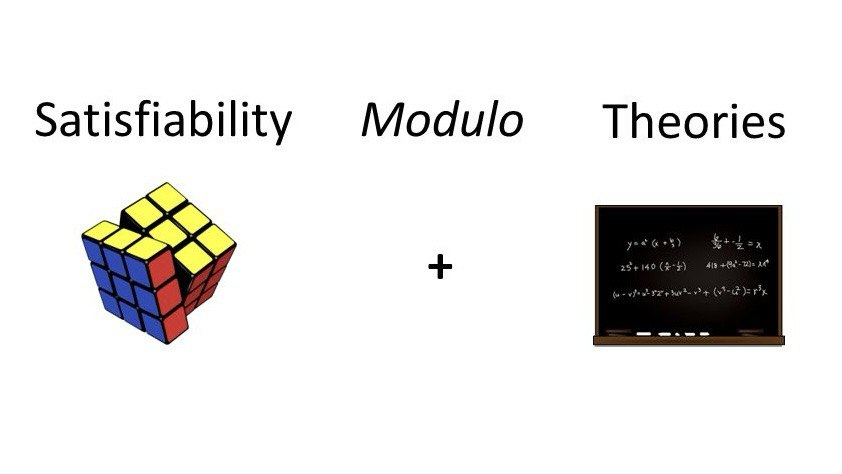
\includegraphics[width=\textheight]{./slides/smt.jpg}
		\end{minipage}
	\end{figure}
    \begin{itemize}
    	\item SMT łączy problem spełnialności logicznej z różnymi teoriami matematycznymi.
    	\item Zadaniem jest stwierdzenie, czy istnieją wartości zmiennych spełniające zarówno ograniczenia logiczne, jak i dodatkowe z teorii matematycznej.
    \end{itemize}
\end{frame}
\begin{frame}{Zastosowanie SMT w praktyce}
	\begin{itemize}
		\item Weryfikacja Mikroprocesorów
		\item Sprawdzanie Równoważności Mikrokodu
		\item Testowanie Biało-Skrzynkowe
		\item Eksploracja Przestrzeni Projektowej
		\item Synteza Konfiguracji
		\item Odkrywanie Materiałów Kombinatorycznych
		\item Problemy NP-Trudne
	\end{itemize}
\end{frame}
\begin{frame}{Problemy NP-trudne}

		 \textbf{Definicja}: Problemy NP-trudne to klasy problemów, które są co najmniej tak trudne jak najtrudniejsze problemy w klasie NP.
		\vspace{10pt}
		
		 \textbf{Klasyfikacja}:
		\begin{itemize}
			\item \textit{Klasa P}: Problemy decyzyjne rozwiązywalne w czasie wielomianowym przez algorytmy deterministyczne.
			\item \textit{Klasa NP}: Problemy, których rozwiązania mogą być zweryfikowane w czasie wielomianowym przez algorytmy niedeterministyczne.
		\end{itemize}
		\vspace{10pt}
		 \textbf{Cechy}:
		\begin{itemize}
			\item Możliwość zredukowania każdego problemu w klasie NP do problemu NP-trudnego w czasie wielomianowym.
			\item Wymagają dużego nakładu obliczeniowego do rozwiązania i weryfikacji, nawet dla relatywnie niewielkich instancji problemów.
		\end{itemize}

\end{frame}
\begin{frame}{SMT solvery}
	\begin{itemize}
		\item Z3
		\item Yices
		\item cvc5
	\end{itemize}
\end{frame}
\begin{frame}{Kodowanie problemów}
\begin{itemize}
\item Każdy problem analizowany w pracy został zamodelowany w postaci bezkwantyfikatorowych formuł logiki pierwszego rzędu jako zestaw ograniczeń logicznych, definiujących jego specyfikację i warunki rozwiązania.
\item W celu przeprowadzenia eksperymentów, problemy zostały zaimplementowane w języku Python, korzystając z wyspecjalizowanej biblioteki Z3. Kodowanie problemów odbyło się zgodnie z formułami.
\item Biblioteka Z3 została wykorzystana do manipulacji oraz rozwiązywania ograniczeń logicznych, co umożliwiło skuteczną implementację algorytmów i procedur rozwiązujących problemy z zakresu kwantyfikacyjnej logiki boolowskiej.
\end{itemize}
\end{frame}
\begin{frame}{Ścieżka Hamiltona w grafie skierowanym}
\textbf{Definicja}
\begin{itemize}
	\item Dany graf skierowany $G = (V, E)$, gdzie $V$ to zbiór wierzchołków, a $E$ to zbiór krawędzi.
	\item Zadaniem jest stwierdzenie, czy graf $G$ zawiera ścieżkę Hamiltona.
	\item Ścieżka Hamiltona to sekwencja wierzchołków $s_0, s_1,…, s_{n−1}$ przechodzącą przez każdy wierzchołek dokładnie raz.	
\end{itemize}
\vspace{10pt}

\textbf{Zastosowania}
\begin{itemize}
	\item Istotny w informatyce, telekomunikacji i bioinformatyce.
	\item Kluczowy dla analizy sieci i trasowania w systemach komunikacyjnych.
\end{itemize}
\end{frame}
\begin{frame}{Ścieżka Hamiltona w grafie skierowanym: Kodowanie}
Używamy $n$ zmiennych $v_0,…,v_{n−1}$, gdzie $n$ to liczba wierzchołków.
\vspace{10pt}

\textbf{Formuły uwzględniające warunki dla zmiennych:}
\vspace{5pt}
\begin{itemize}
	\item Zakres zmiennych $v_j$: $\propernumbers(n) = \left( \bigwedge_{j=0}^{n-1} (v_j \geq 0 \land v_j < n) \right) $.
	\item Unikalność zmiennych: $\distinctvs(n) = \left( \bigwedge_{i=0}^{n-1} \bigwedge_{j=i+1}^{n} (v_i \neq v_j) \right)$.
	\item Sprawdzenie krawędzi grafu: $\diredges(n,E) = \left( \bigwedge_{i=0}^{n-1} \bigvee_{(s,t) \in E} (v_i = s \land v_{i+1} = t) \right)$.
\end{itemize}
\vspace{10pt}
\textbf{Cała Formuła:}
\begin{align*}
	\HamPath(n, E) = \propernumbers(n) \land \distinctvs(n) \land \diredges(n, E)
\end{align*}
\end{frame}
\begin{frame}{Ścieżka Hamiltona w grafie nieskierowanym}
	\textbf{Warunki dla zmiennych:}
\begin{itemize}
	\item Zakres zmiennych $v_j$: $\propernumbers(n)$.
	\item Unikalność zmiennych: $\distinctvs(n)$.
	\item Możliwość przechodzenia przez krawędź w obie strony: $\edges(n, E) = \left( \bigwedge_{i=0}^{n-1} \bigvee_{\{s,t\} \in E} (v_i = s \land v_{i+1} = t) \lor (v_i = t \land v_{i+1} = s) \right)$.
\end{itemize}
\vspace{10pt}
	
\textbf{Formuła:}
\begin{align*}
	\UHamPath(n, E) = \propernumbers(n) \land \distinctvs(n) \land \edges(n, E)
\end{align*}
\end{frame}
\begin{frame}{Problem maksymalnej kliki w grafie nieskierowanym}
\textbf{Definicja}
\begin{itemize}
	\item Dany graf nieskierowany $G = (V, E)$, gdzie $V$ to zbiór wierzchołków, $E$ to zbiór krawędzi.
	\item Klika to pełny podgraf, gdzie każde dwa wierzchołki są połączone krawędzią.
	\item Maksymalna klika $C \subseteq V$  to taka, która zawiera największą możliwą liczbę wierzchołków.
\end{itemize}
\vspace{10pt}

\textbf{Zastosowania}
\begin{itemize}
	\item Istotny w teorii grafów, sieciach społecznościowych, analizie sieci.
	\item Wykorzystywany w problemach planowania tras, optymalizacji sieci, analizie zależności między obiektami.
\end{itemize}
\end{frame}
	
\begin{frame}{Problem maksymalnej kliki w grafie nieskierowanym: Kodowanie}
Używamy $k$ zmiennych $v_0,…,v_{k−1}$, gdzie $0 < k \leq n$.
\vspace{10pt}
	
\textbf{Warunki dla zmiennych:}
\vspace{5pt}
\begin{itemize}
	\item Zakres zmiennych $v_j$: $\propernumbers(n)$.
	\item Unikalność zmiennych: $\distinctvs(n)$.
	\item Każda para zmiennych $v_i$ i	$v_j$ jest połączona krawędzią.	
\end{itemize}
\vspace{10pt}
	\textbf{Formuła:}
\begin{align*}
	&\MaxClique(n, E, k) = \propernumbers(k)  \land \distinctvs(k)  \land \\
	&\left( \bigwedge_{i=0}^{k-1} \bigwedge_{j=i+1}^{k} \bigvee_{\{s,t\} \in E} ((v_i = s \land v_j = t) \lor (v_j = s \land v_i = t)) \right)	
\end{align*}
\end{frame}
	
\begin{frame}{Problem maksymalnego zbioru niezależnego w grafie nieskierowanym}
\textbf{Definicja}
\begin{itemize}
	\item Dany graf nieskierowany $G = (V, E)$, gdzie $V$ to zbiór wierzchołków, $E$ to zbiór krawędzi.
	\item Niezależny zbiór to podzbiór wierzchołków, gdzie żadne dwa nie sąsiadują ze sobą.
	\item Problem maksymalnego zbioru niezależnego polega na znalezieniu największego takiego zbioru w grafie.
\end{itemize}
\vspace{10pt}

\textbf{Zastosowania}
\begin{itemize}
	\item Istotny w teorii grafów i algorytmice.
	\item Ma zastosowanie w wielu problemach optymalizacyjnych i analizie sieci.
\end{itemize}
\end{frame}
	
\begin{frame}{Problem maksymalnego zbioru niezależnego w grafie nieskierowanym: Kodowanie}
Używamy $n$ zmiennych $v_0,…,v_{n−1}$, gdzie $n$ to liczba wierzchołków w grafie.
\vspace{10pt}

\textbf{Warunki dla zmiennych:}
\vspace{5pt}
\begin{itemize}
	\item Zakres zmiennych $v_j$: $\propernumbers(n)$.
	\item Unikalność zmiennych: $\distinctvs(n)$.
	\item Brak krawędzi między wierzchołkami.
\end{itemize}
\vspace{10pt}
\textbf{Formuła:}
\begin{align*}
	\MaxIndSet(n, E, k) = \propernumbers(n) \land \distinctvs(n)  \land \\
	\left( \bigwedge_{i=0}^{k-1} \bigwedge_{j=i+1}^{k} \bigvee_{\{s,t\} \in E} \lnot((v_i = s \land v_j = t) \lor (v_j = s \land v_i = t)) \right)	
\end{align*}
\end{frame}
	
\begin{frame}{Problem pokrycia wierzchólkowego}
\textbf{Definicja}
\begin{itemize}
	\item Pokrycie wierzchołkowe grafu nieskierowanego	$G = (V, E)$ to podzbiór $V'\subseteq V$, gdzie każda krawędź ma przynajmniej jeden koniec w $V'$.
	\item Rozmiar pokrycia to liczba wierzchołków w nim zawartych.
	\item Problem polega na znalezieniu minimalnego pokrycia wierzchołkowego w danym grafie.
\end{itemize}
\vspace{10pt}

\textbf{Zastosowania}
\begin{itemize}
	\item Istotny w optymalizacji grafów oraz problemach planowania tras.
	\item Stosowany w analizie sieci, zarządzaniu zasobami oraz problemach pokrycia.
\end{itemize}
\end{frame}
\begin{frame}{Problem pokrycia wierzchólkowego: Kodowanie}
Używamy $k$ zmiennych $v_0,…,v_{k−1}$, gdzie $0 < k \leq n$.
\vspace{10pt}

\textbf{Warunki dla zmiennych:}
\vspace{5pt}
\begin{itemize}
	\item Zakres zmiennych $v_j$: $\propernumbers(k)$.
	\item Unikalność zmiennych: $\distinctvs(k)$.
	\item Dla każdej krawędzi w $E$ co najmniej jeden z jej końców należy do $V'$.
\end{itemize}
\vspace{10pt}

\textbf{Formuła:}
\begin{align*}
	\VertexCover&(n, E, k) = \propernumbers(k) \land \distinctvs(k) \land \\
	&\left( \bigwedge_{\{s,t\} \in E} (\bigvee_{j=0}^{k-1} (v_j = s \lor v_j = t)) \right)	
\end{align*}
\end{frame}
\begin{frame}{Problem kolorowania grafu}
\textbf{Definicja}
\begin{itemize}
	\item Problem polega na określeniu minimalnej liczby kolorów potrzebnych do pokolorowania grafu nieskierowanego $G = (V, E)$.
	\item Dwa sąsiednie wierzchołki nie mogą mieć tego samego koloru.	
\end{itemize}
\vspace{10pt}

\textbf{Zastosowania}
\begin{itemize}
	\item Modelowanie problemu kolorowania map za pomocą grafu, w którym każdy wierzchołek reprezentuje kraj, i wierzchołki, których kraje mają wspólną granicę, ze sobą sąsiadują.
	\item Istotny w planowaniu tras, optymalizacji sieci oraz problemach planowania.
\end{itemize}
\end{frame}
\begin{frame}{Problem kolorowania grafu: Kodowanie}
Używamy $n$ zmiennych $c_0,…,c_{n−1}$​,gdzie $n$ to liczba wierzchołków w grafie.
\vspace{10pt}

\textbf{Warunki dla zmiennych:}
\vspace{5pt}
\begin{itemize}
	\item Każda zmienna $c_j$ reprezentująca kolor wierzchołka $j$ przyjmuje wartość z przedziału od $1$ do $k$, gdzie $k$ to liczba kolorów.
	\item Dla każdej krawędzi $s,t$ w $E$, kolor wierzchołka $s$ jest różny od koloru wierzchołka $t$.
\end{itemize}
\vspace{10pt}

\textbf{Formuła:}
\begin{align*}
	\GraphColoring(n, E) = \left( \bigwedge_{j=1}^{n} (c_j \geq 1 \land c_j \leq k) \right) \land 
	\left( \bigwedge_{\{s,t\} \in E} (c_s \neq c_t) \right)
\end{align*}	
\end{frame}
\begin{frame}{Problem Komiwojażera}
\textbf{Definicja}
\begin{itemize}
	\item Problem polega na znalezieniu trasy, która minimalizuje sumaryczny koszt podróży, odwiedzając każde miasto dokładnie raz i kończąc w mieście początkowym.
	\item Dany graf nieskierowany $G = (V, E)$, gdzie wierzchołki reprezentują miasta, a krawędzie odpowiadają możliwym połączeniom między nimi.
	Koszt podróży z miasta $i$ do $j$ jest reprezentowany przez wagę $c(i,j)$.
	\item Celem jest znalezienie trasy o minimalnym koszcie, która odwiedza każde miasto dokładnie raz.
\end{itemize}
\vspace{10pt}

\textbf{Zastosowania}
\begin{itemize}
	\item Logistyka, planowanie tras, optymalizacja sieci komunikacyjnych.
\end{itemize}
\end{frame}
\begin{frame}{Problem Komiwojażera: Kodowanie}
Używamy $n$ zmiennych $v_0,…, v_{n−1}$, gdzie $n$ to liczba miast.
\vspace{10pt}

\textbf{Warunki dla zmiennych:}
\vspace{5pt}
\begin{itemize}
	\item Właściwą wartość i unikalność.
	\item Istnienie krawędzi między kolejnymi wierzchołkami w trasie oraz zamknięcie trasy.
	\item Ograniczenie sumy wag krawędzi na trasie do wartości $k$.
\end{itemize}

\vspace{10pt}
\textbf{Formuła:}	
\begin{align*}
	&\TSP(n, c, E, k) = \propernumbers(n) \land \distinctvs(n) \land \edges(n, E)  \\
	&\land \left( \bigvee_{\{s,t\} \in E} ((v_{n-1} = s \land v_0 = t) \lor (v_0 = s \land v_{n-1} = t)) \right) \land 
	\left( \bigwedge_{\{s,t\} \in E} \sum c(s,t) \leq k \right)
\end{align*}
	
\end{frame}
\begin{frame}{Problem sumy podzbioru}
\textbf{Definicja}
\begin{itemize}
	\item Problem sumy podzbioru polega na znalezieniu podzbioru $S' \subseteq S$, którego elementy sumują się dokładnie do wartości docelowej $t$. 
\end{itemize}
\vspace{10pt}

\textbf{Zastosowania}
\begin{itemize}
	\item Wykorzystywany w optymalizacji kombinatorycznej, analizie danych oraz w algorytmach szukających rozwiązań problemów optymalizacyjnych.
	\item Stosowany w bioinformatyce do analizy sekwencji genetycznych.
	\item W praktyce wykorzystywany w planowaniu finansowym, analizie portfela inwestycyjnego, czy w układaniu harmonogramów.
\end{itemize}	
\end{frame}
	
\begin{frame}{Problem sumy podzbioru: Kodowanie}
Używamy $n$ zmiennych $x_0,…, x_{n−1}$, gdzie $n$ to liczba elementów w $S$.
\vspace{10pt}

\textbf{Warunki dla zmiennych:}
\vspace{5pt}
\begin{itemize}
	\item każda zmienna $x_j$ przyjmuje wartość logiczną $0$ lub $1$.
	\item suma iloczynów $x_i$ i $s_i$ dla wszystkich $k$ elementów ze zbioru $S$ jest równa wartości $t$.
\end{itemize}
\vspace{10pt}

\textbf{Formuła:}
\begin{align*}
	\SubsetSum(n, t) = \left( \bigwedge_{j=0}^{n-1} (x_j = 0 \lor x_j = 1) \right) \land 
	\left( \sum_{i=0}^{n} (x_i * s_i) = t \right)
\end{align*}
\end{frame}
	
\begin{frame}{Generowanie danych wejściowych}
	\begin{itemize}
		\item Do eksperymentów użyto laptopa Dell z procesorem Intel Core i5-1135G7 z częstotliwością 2.40GHz i 16 GB RAMu.
		\item Generowanie danych wejściowych, takich jak grafy, wykonano przy użyciu biblioteki igraph, która zapewnia wszechstronne możliwości manipulacji i analizy grafów.
		
		\item Zdecydowano się generować dwa rodzaje grafów - Barabasi-Alberta i Erdos-Rényi’ego - aby umożliwić badanie efektywności SMT-solverów w różnych warunkach.
		
		\item Do eksperymentów nad problemem SubsetSum wygenerowano zestawy losowych liczb całkowitych w określonym zakresie.
		
	\end{itemize}
\end{frame}
	
\begin{frame}{Wyniki dla Ścieżki Hamiltona w grafie skierowanym}
\begin{figure}[htbp]
	\centering
	\begin{subfigure}[b]{0.5\textwidth}
		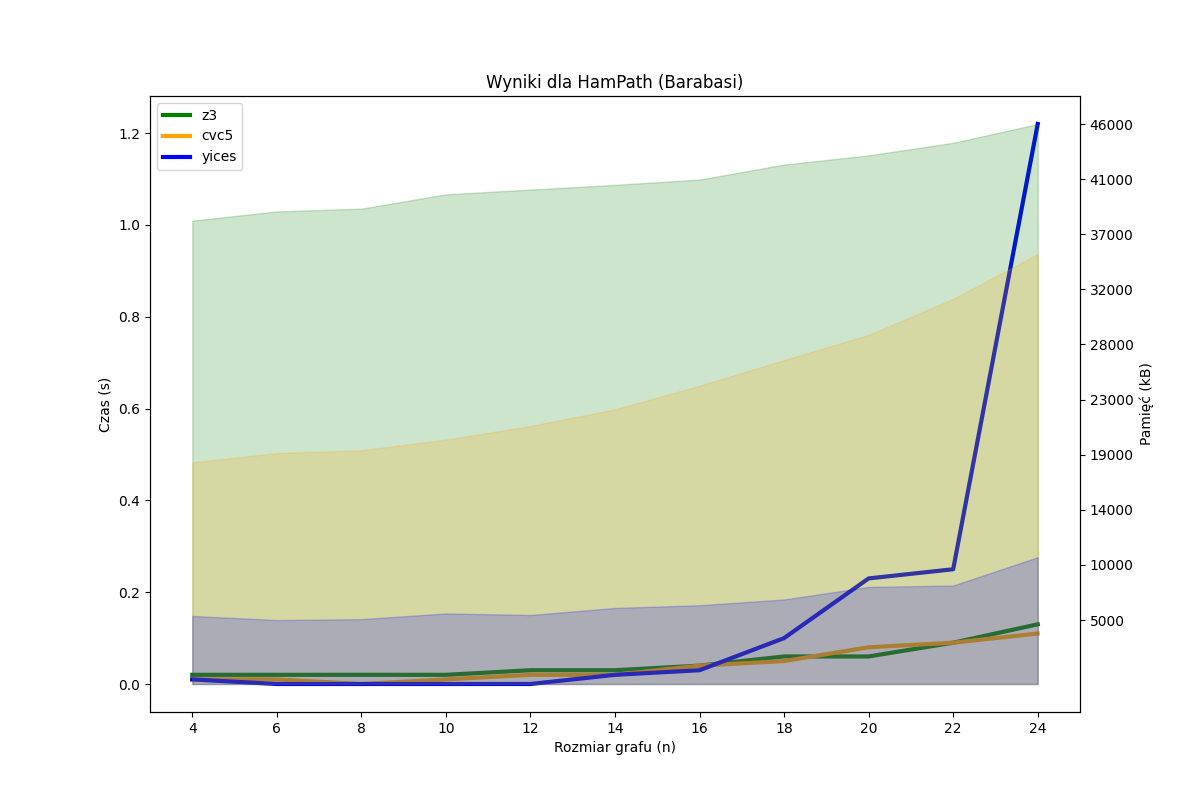
\includegraphics[width=\textwidth]{../thesis/figures/1-barabasi-plot.png}
	\end{subfigure}
	\begin{subfigure}[b]{0.49\textwidth}
		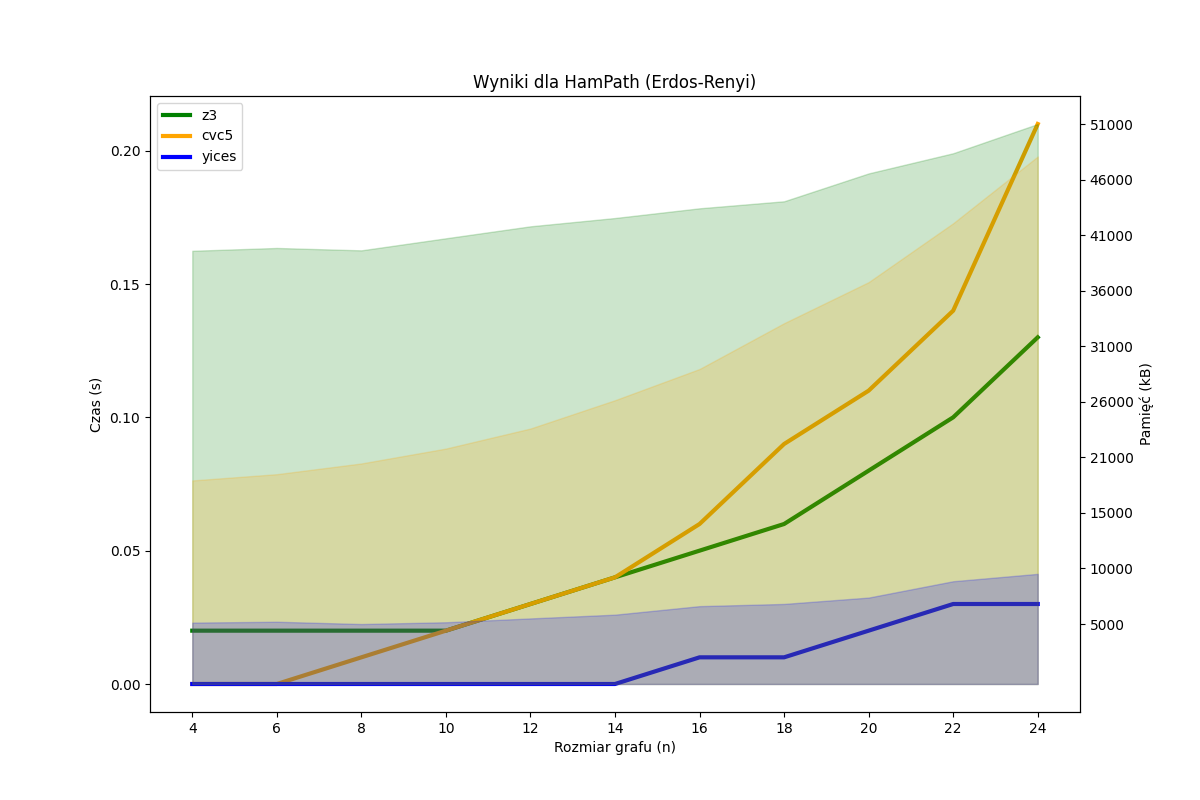
\includegraphics[width=\textwidth]{../thesis/figures/1-erdos-renyi-plot.png}
	\end{subfigure}
\end{figure}
\end{frame}
	
\begin{frame}{Wyniki dla Ścieżki Hamiltona w grafie nieskierowanym}
	\begin{figure}[htbp]
		\centering
		\begin{subfigure}[b]{0.5\textwidth}
			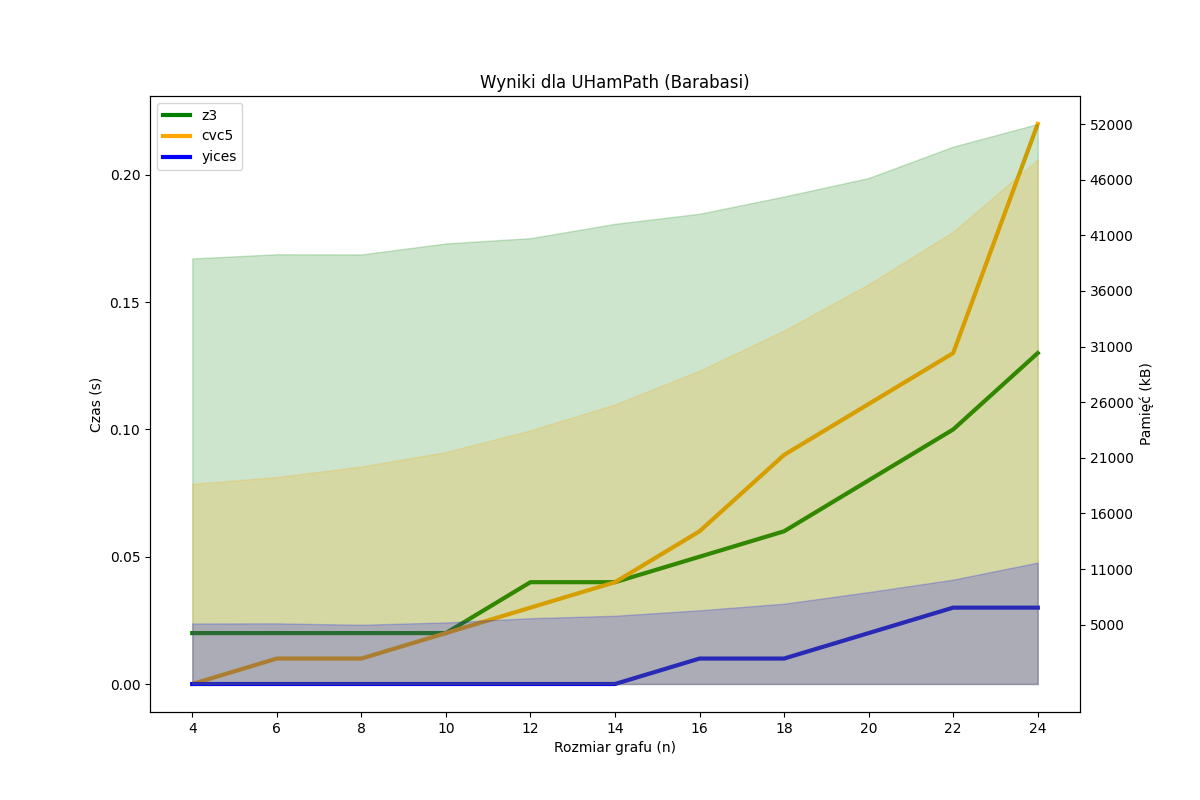
\includegraphics[width=\textwidth]{../thesis/figures/2-barabasi-plot.png}
		\end{subfigure}
		\begin{subfigure}[b]{0.49\textwidth}
			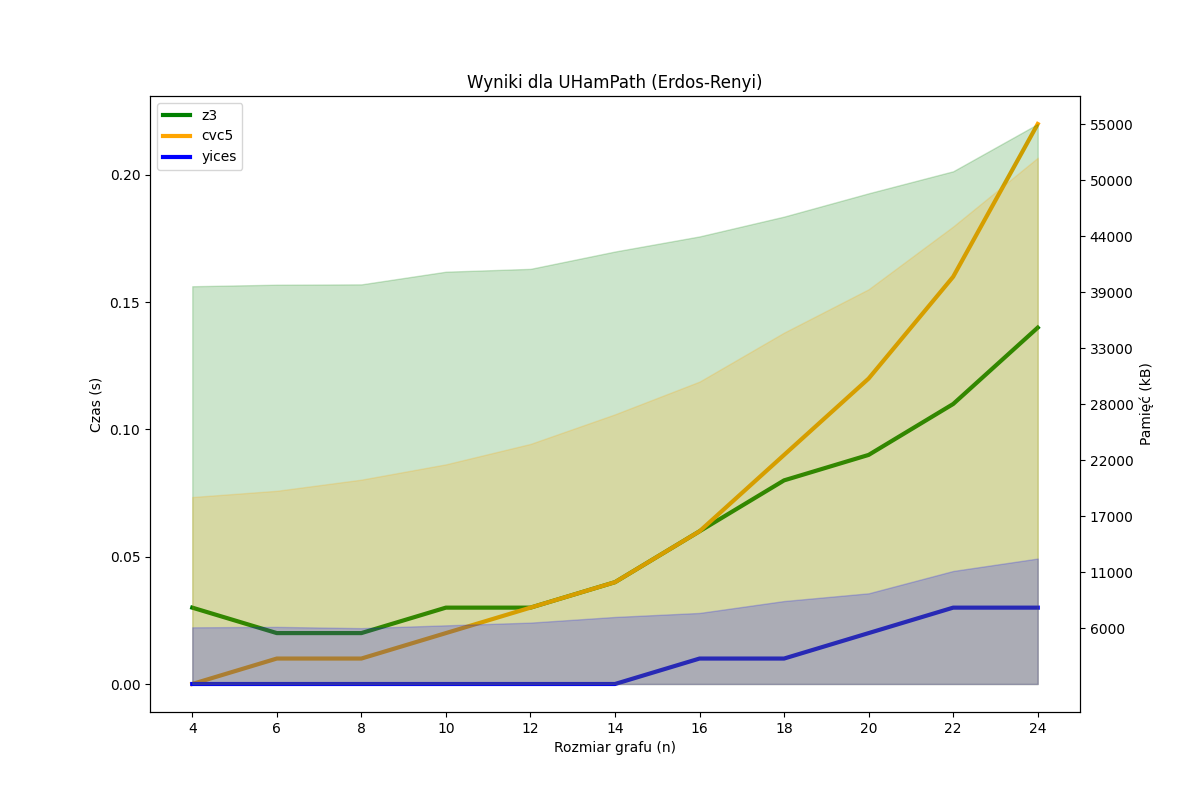
\includegraphics[width=\textwidth]{../thesis/figures/2-erdos-renyi-plot.png}
		\end{subfigure}
	\end{figure}
\end{frame}
	
\begin{frame}{Wyniki dla Problemu maksymalnej kliki}
	\begin{figure}[htbp]
		\centering
		\begin{subfigure}[b]{0.5\textwidth}
			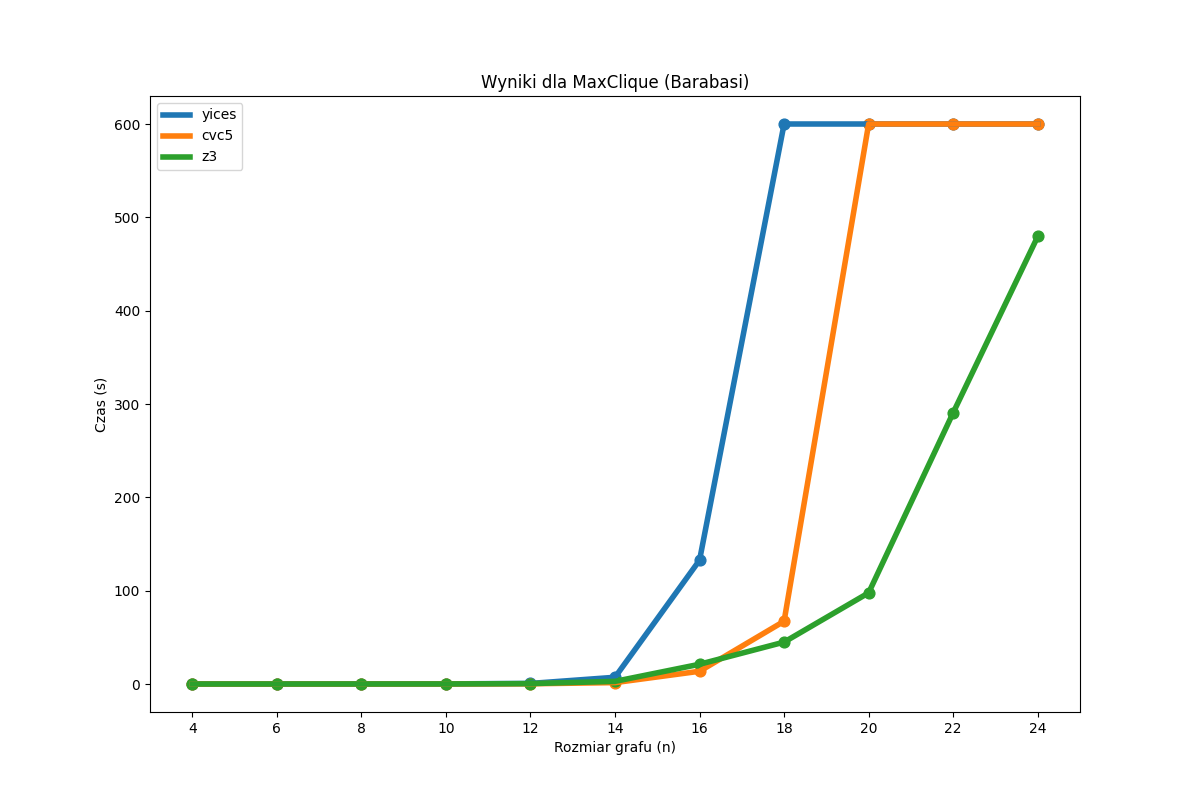
\includegraphics[width=\textwidth]{../thesis/figures/3-barabasi-plot.png}
		\end{subfigure}
		\begin{subfigure}[b]{0.49\textwidth}
			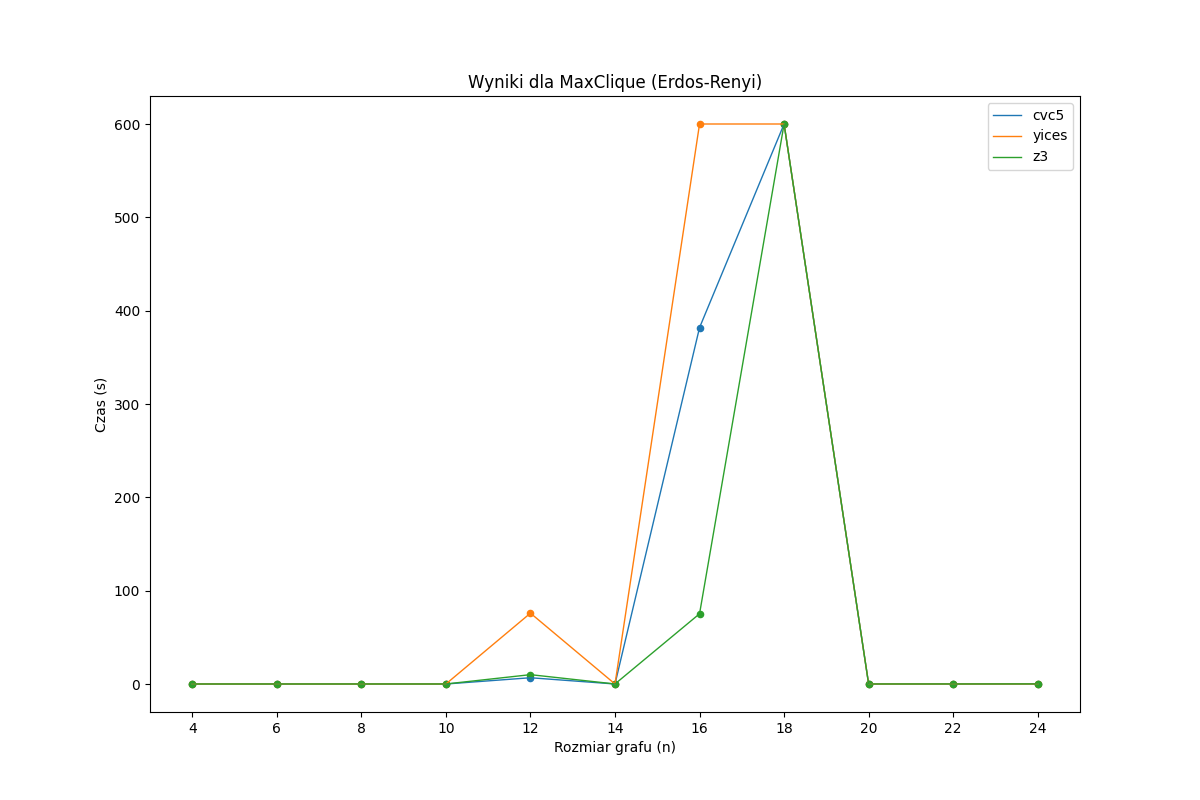
\includegraphics[width=\textwidth]{../thesis/figures/3-erdos-renyi-plot.png}
		\end{subfigure}
	\end{figure}
\end{frame}
	
\begin{frame}{Wyniki dla Problemu maksymalnego zbioru niezależnego}
	\begin{figure}[htbp]
		\centering
		\begin{subfigure}[b]{0.5\textwidth}
			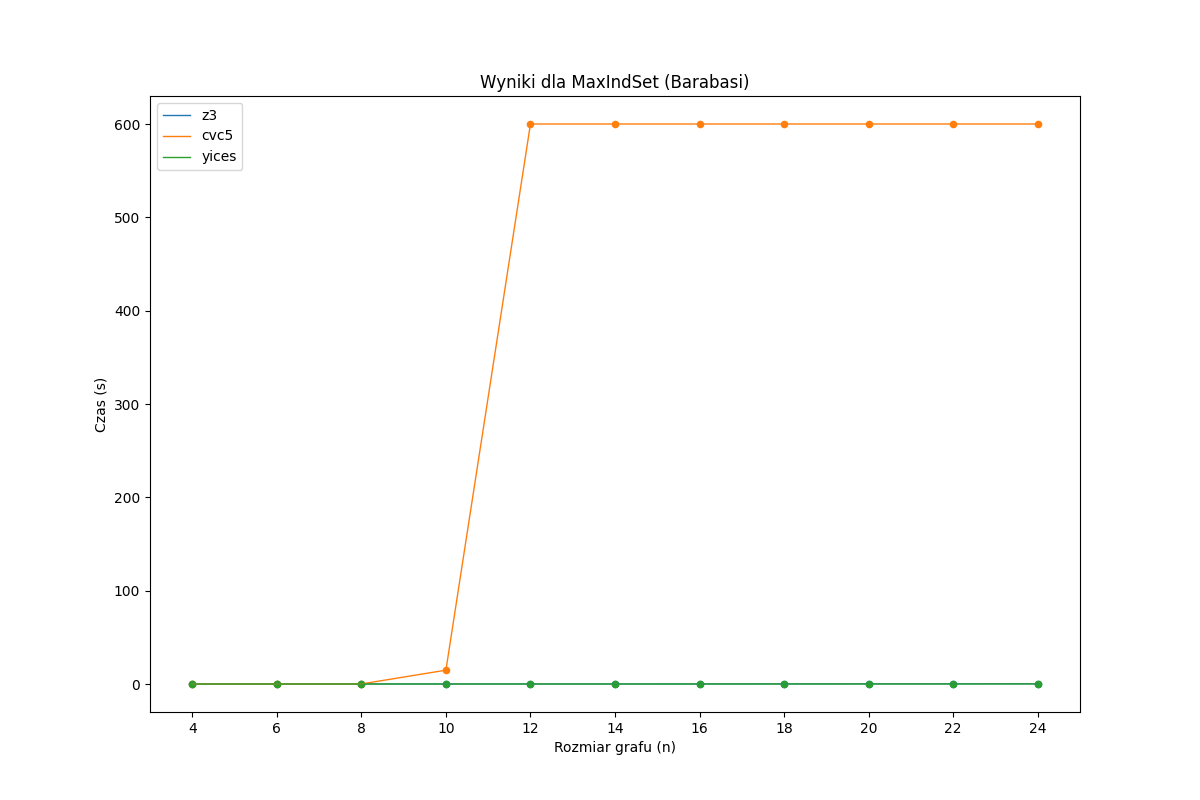
\includegraphics[width=\textwidth]{../thesis/figures/4-barabasi-plot.png}
		\end{subfigure}
		\begin{subfigure}[b]{0.49\textwidth}
			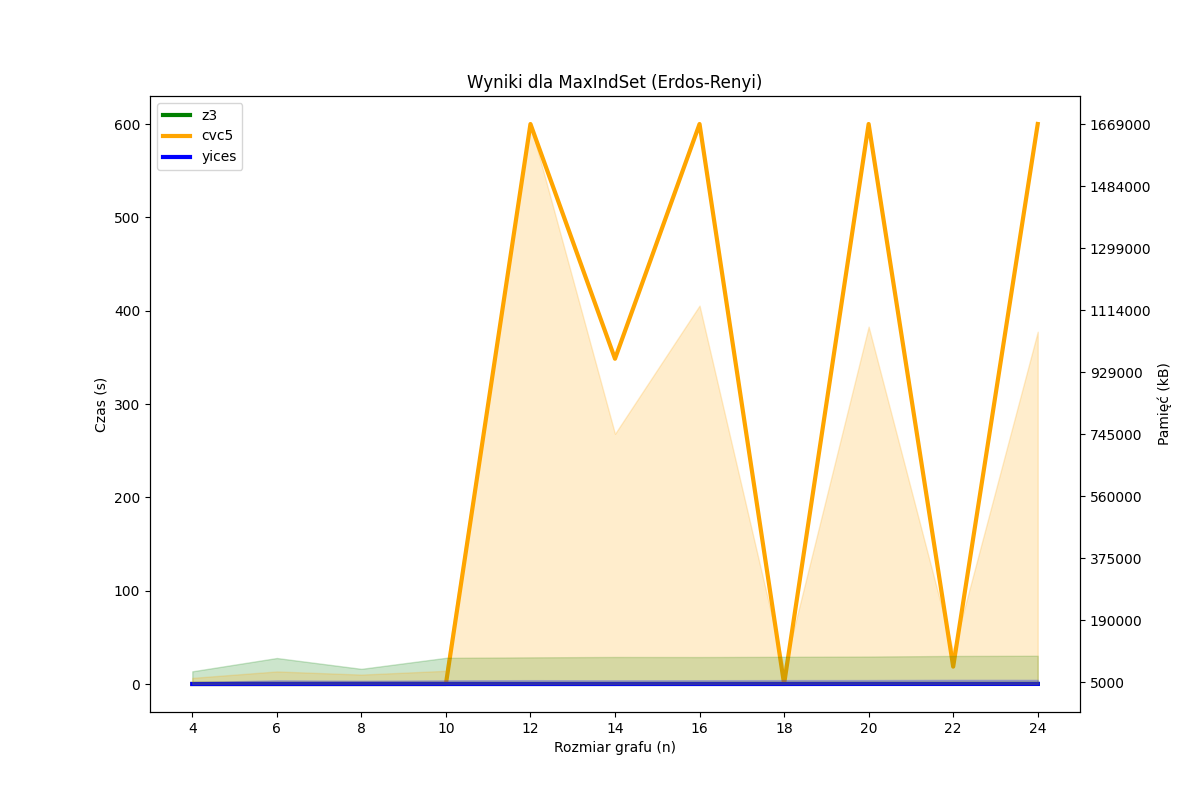
\includegraphics[width=\textwidth]{../thesis/figures/4-erdos-renyi-plot.png}
		\end{subfigure}
	\end{figure}
\end{frame}
	
\begin{frame}{Wyniki dla Problemu pokrycia wierzchołkowego}
	\begin{figure}[htbp]
		\centering
		\begin{subfigure}[b]{0.5\textwidth}
			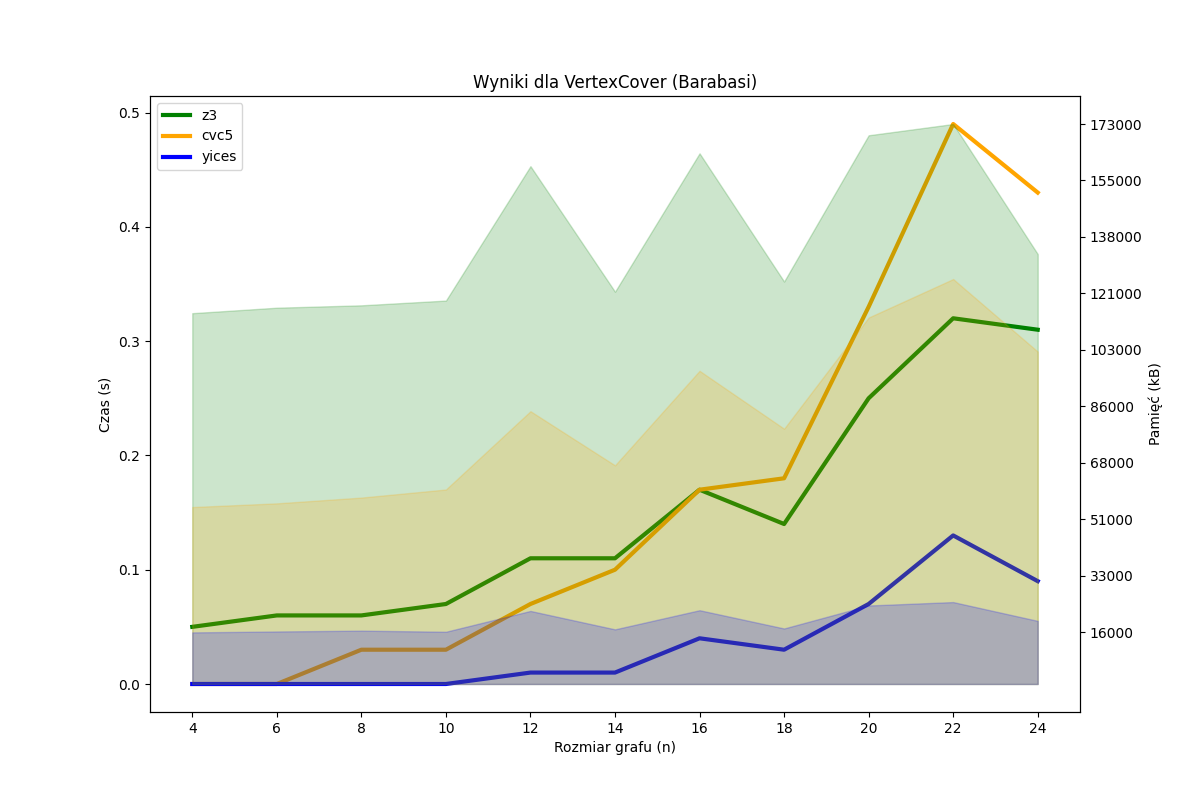
\includegraphics[width=\textwidth]{../thesis/figures/5-barabasi-plot.png}
		\end{subfigure}
		\begin{subfigure}[b]{0.49\textwidth}
			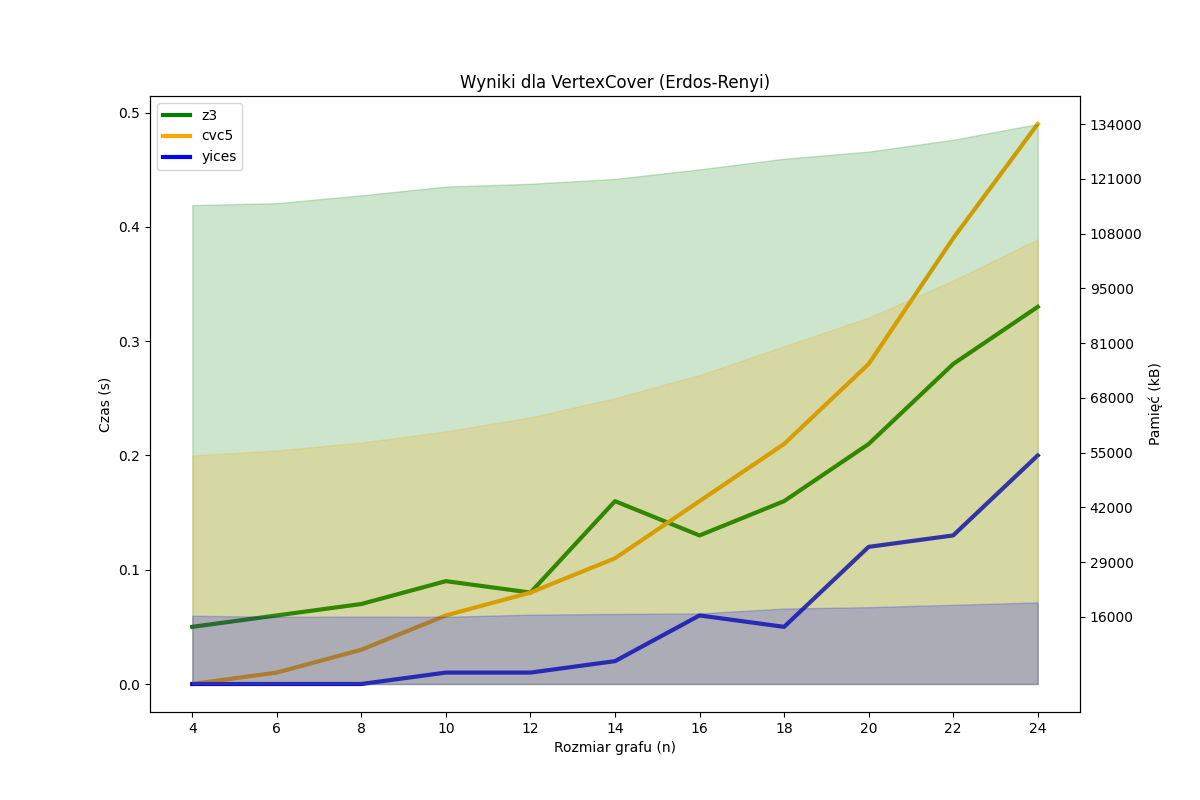
\includegraphics[width=\textwidth]{../thesis/figures/5-erdos-renyi-plot.png}
		\end{subfigure}
	\end{figure}
\end{frame}
	
\begin{frame}{Wyniki dla Problemu kolorowania grafu}
	\begin{figure}[htbp]
		\centering
		\begin{subfigure}[b]{0.5\textwidth}
			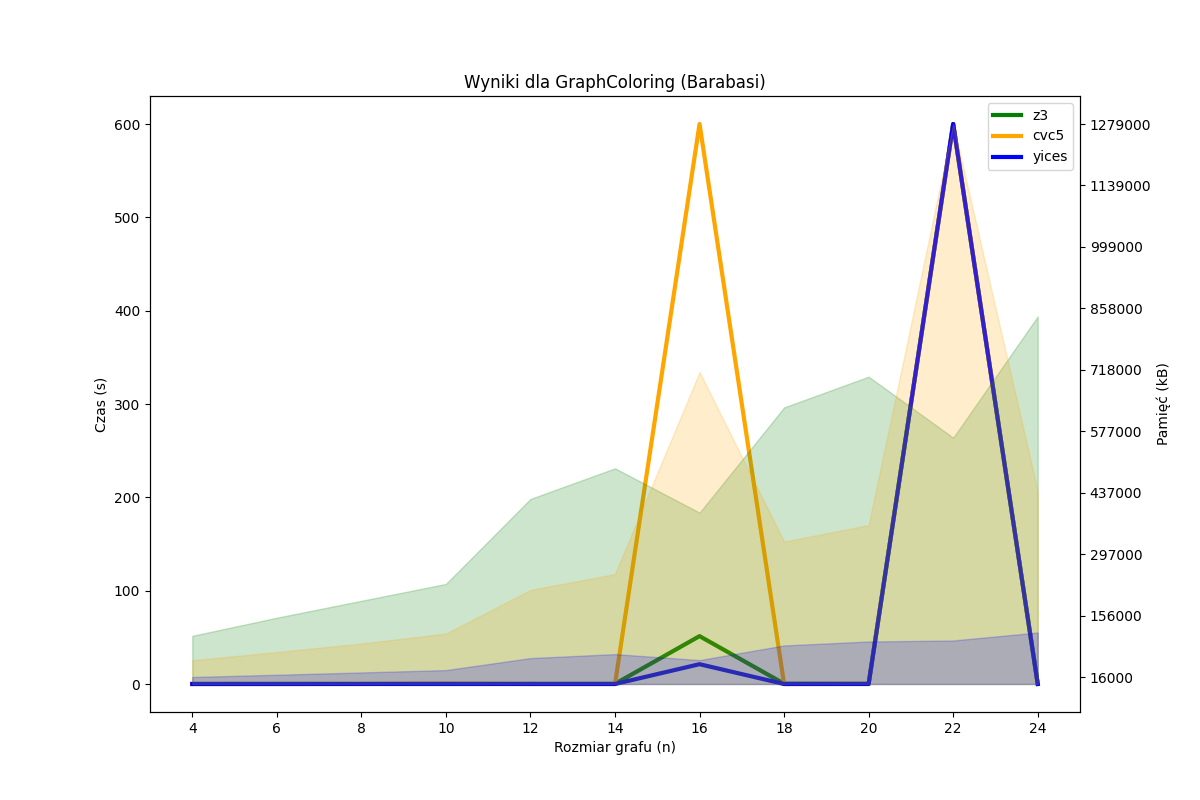
\includegraphics[width=\textwidth]{../thesis/figures/6-barabasi-plot.png}
		\end{subfigure}
		\begin{subfigure}[b]{0.49\textwidth}
			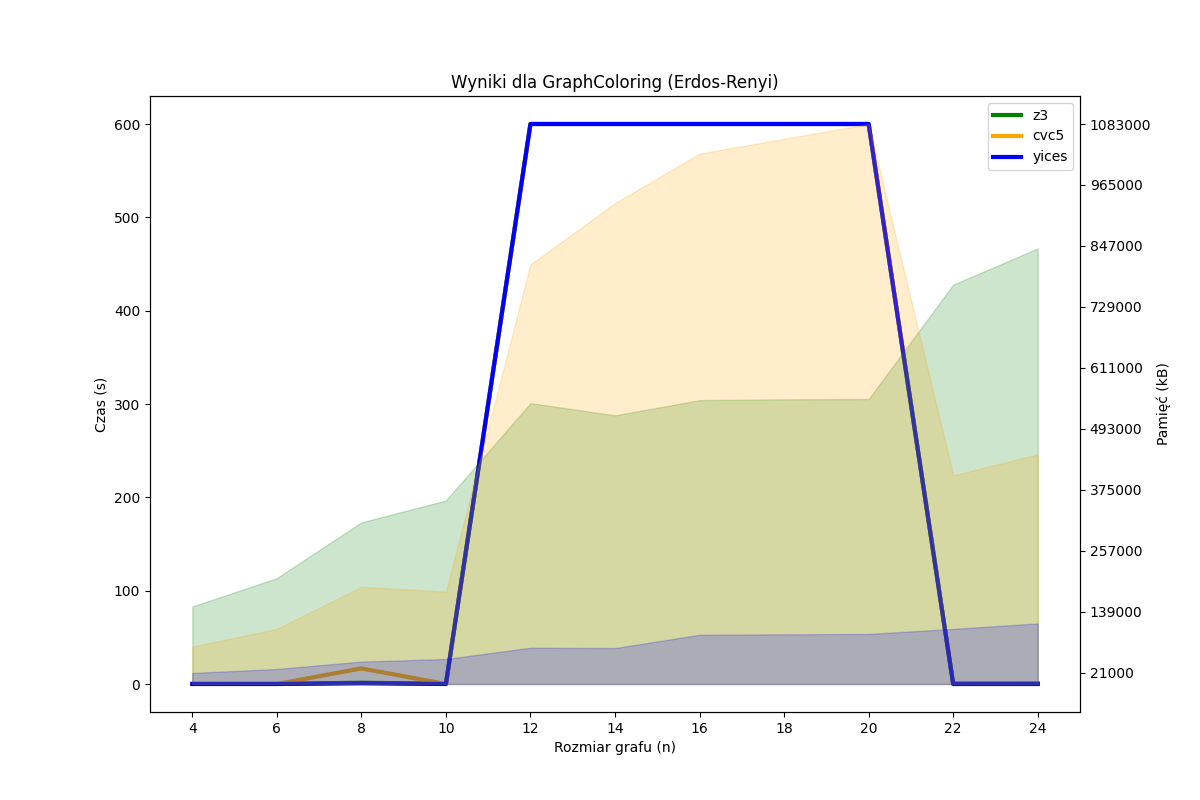
\includegraphics[width=\textwidth]{../thesis/figures/6-erdos-renyi-plot.png}
		\end{subfigure}
	\end{figure}
\end{frame}
	
\begin{frame}{Wyniki dla Problemu Komiwojażera}
	\begin{figure}[htbp]
		\centering
		\begin{subfigure}[b]{0.5\textwidth}
			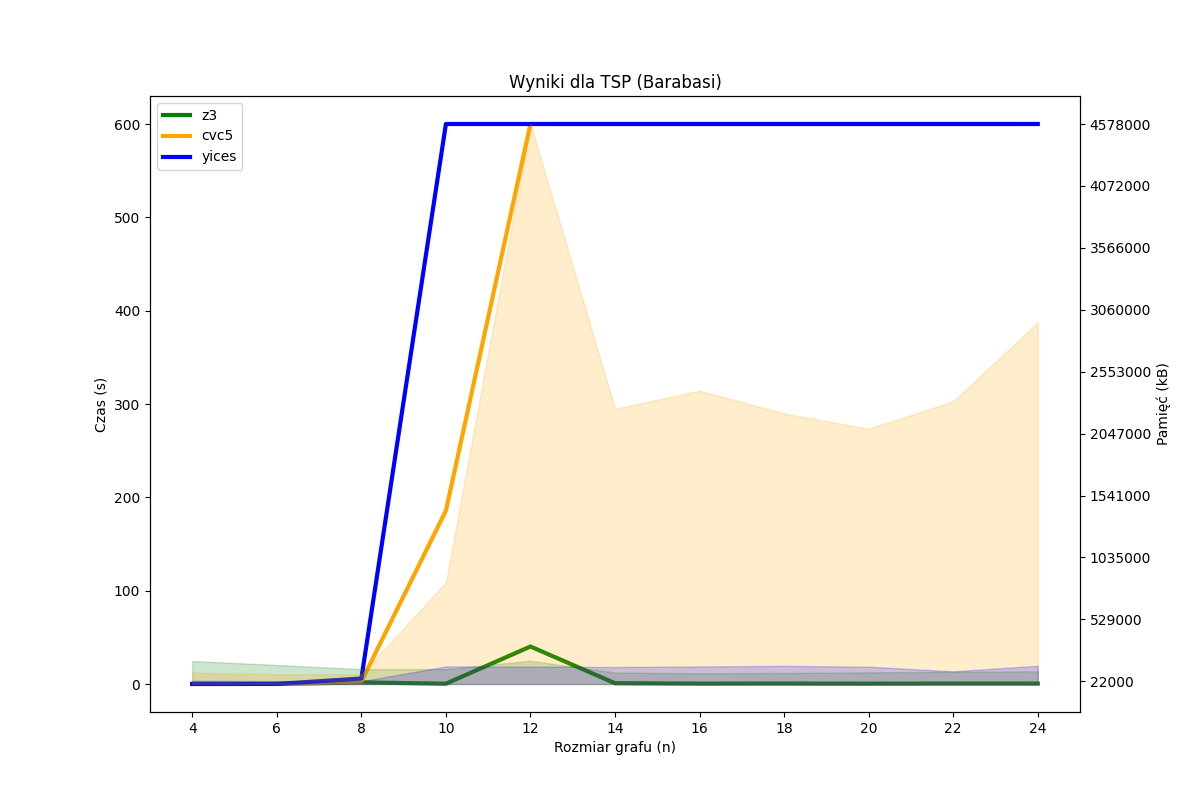
\includegraphics[width=\textwidth]{../thesis/figures/7-barabasi-plot.png}
		\end{subfigure}
		\begin{subfigure}[b]{0.49\textwidth}
			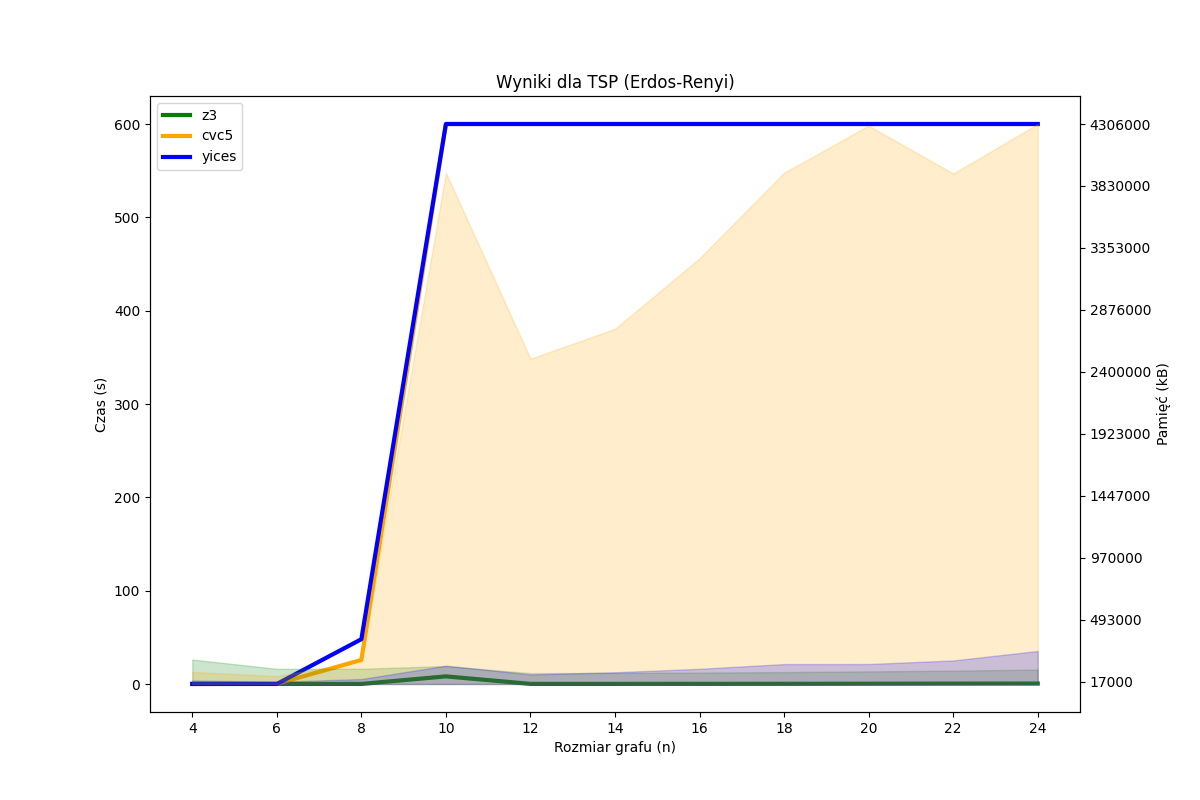
\includegraphics[width=\textwidth]{../thesis/figures/7-erdos-renyi-plot.png}
		\end{subfigure}
	\end{figure}
\end{frame}
	
\begin{frame}{Wyniki dla Problemu sumy podzbioru}
	\begin{figure}[htbp]
		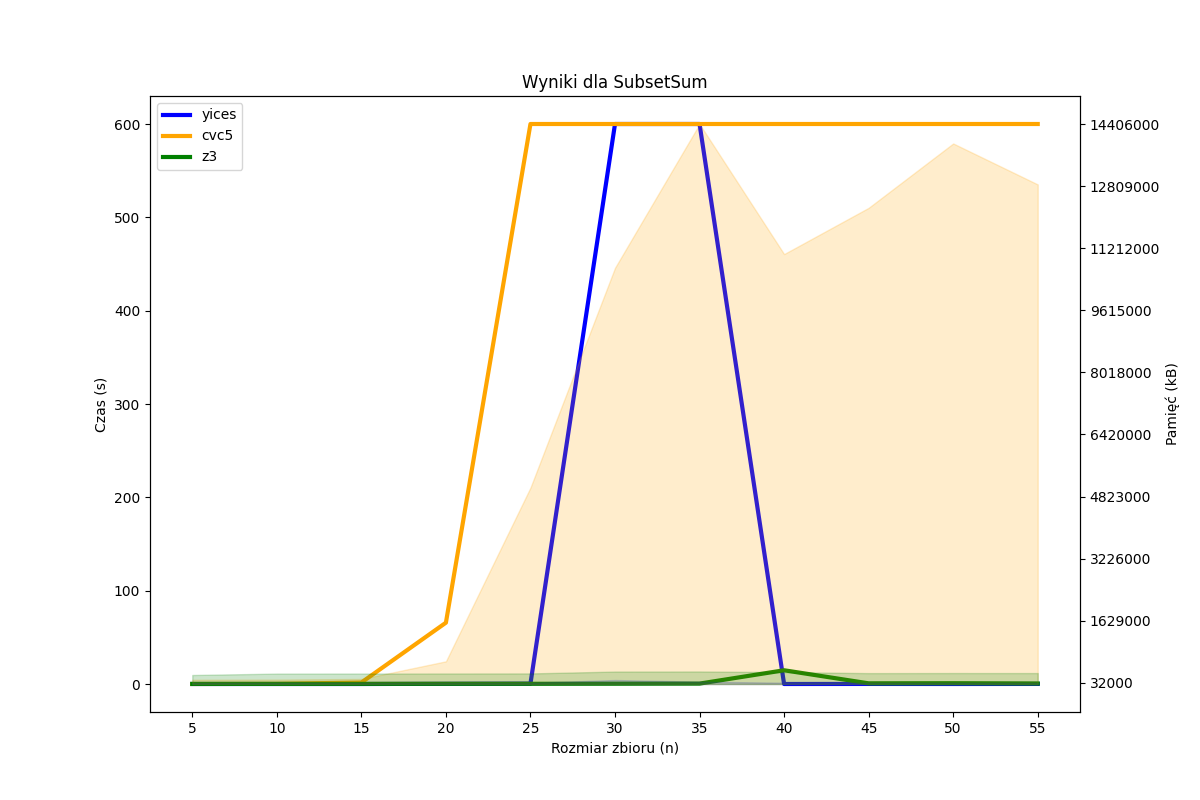
\includegraphics[width={0.9\textwidth}]{../thesis/figures/8-plot.png}
	\end{figure}
\end{frame}
	
\begin{frame}{Identyfikacja czynników wpływających na efektywność}
	\begin{itemize}
		\item Rozmiar Instancji Problemu:
		Wraz z rosnącym rozmiarem problemu, np. liczbą wierzchołków w grafie lub elementów w zbiorze, czas rozwiązania znacząco wzrasta.
		\item Struktura Grafu:
		Sposób generowania grafu oraz jego złożoność mogą wpływać na wydajność obliczeniową solverów.
		\item Rodzaj Problemu:
		Różnice w wydajności solverów zależą od rodzaju problemu NP-trudnego, np. SubsetSum vs. problemy grafowe.
		\item Zużycie Zasobów:
		Wartość czasowa i pamięciowa solverów różni się w zależności od problemu oraz zastosowanej strategii rozwiązania.
		\item Trudność Spełnialności vs. Niespełnialności:
		Szukanie niespełnialności może być trudniejsze niż spełnialności, co wpływa na czasochłonność rozwiązania problemu.
	\end{itemize}
\end{frame}
	
\begin{frame}{Wnioski}
	Po przeprowadzeniu eksperymentów oraz analizie czynników wpływających na efektywność solverów w rozwiązywaniu problemów NP-trudnych, można wyciągnąć kilka istotnych wniosków:
	\begin{itemize}
		\item Solver Z3 wykazał się jako najbardziej uniwersalny i efektywny w rozwiązywaniu różnorodnych problemów NP-trudnych.
		
		\item Przy rozwiązywaniu problemów NP-trudnych ważne jest efektywne zarządzanie zasobami pamięciowymi.		
	\end{itemize}
\vspace{10pt}
Wnioski te mogą być przydatne dla praktyków oraz badaczy zajmujących się problemami NP-trudnymi, pomagając im wybrać odpowiedni solver oraz zoptymalizować proces rozwiązywania problemów w praktyce.

\end{frame}

\begin{frame}{Podsumowanie}
\begin{itemize}
	\item Dzięki analizie eksperymentalnej zyskałam głębsze zrozumienie wydajności solverów SMT w różnych scenariuszach, co jest istotne zarówno dla praktyki, jak i badań naukowych. 
	\item Wyzwaniem naukowym jest rozwój kodowania szerszej gamy problemów NP-trudnych i przeprowadzenie eksperymentów na bardziej zróżnicowanych danych wejściowych. To pozwoliłoby na pełniejsze zrozumienie możliwości i ograniczeń solverów SMT oraz ich praktyczne zastosowanie.
	\item Wszystkie pliki, kod źródłowy, eksperymenty i inne zasoby związane z niniejszą pracą znajdują się na platformie GitHub.
\end{itemize}
\end{frame}
	

\end{document}